% Lecture notes for the demo library (e2e/demo/README.md): written for
% paperus, in two columns, so fluent mode has something to show.
\documentclass[10pt,twocolumn]{article}
\usepackage[a4paper,margin=18mm,columnsep=7mm]{geometry}
\usepackage[T1]{fontenc}
\usepackage{lmodern}
\usepackage{amsmath,amssymb}
\usepackage{tikz}
\usepackage[hidelinks,pdftitle={The quantum harmonic oscillator},pdfauthor={Mira Kessler}]{hyperref}

\newcommand{\ad}{a^\dagger}
\newcommand{\ket}[1]{\lvert #1\rangle}
\newcommand{\bra}[1]{\langle #1\rvert}

\title{\bfseries The quantum harmonic oscillator}
\author{Mira Kessler\\\small Theory group, lecture notes for Quantum Mechanics II}
\date{Winter term 2026/27, lecture 4}

\begin{document}
\maketitle

\begin{abstract}
The harmonic oscillator is the one problem every quantum physicist solves
twice: once with differential equations and once with operators. These
notes take the second route. We introduce the ladder operators, derive the
evenly spaced spectrum and the ground state, and close with coherent
states, the quantum states that move most like a classical pendulum.
\end{abstract}

\section{Why the oscillator}

Near the bottom of almost any smooth potential, the energy grows with the
square of the distance from the minimum. Expanding $V(x)$ around $x_0$
gives
\begin{equation}
  V(x) \approx V(x_0) + \tfrac12 V''(x_0)\,(x-x_0)^2 ,
\end{equation}
so small vibrations of molecules, phonons in a crystal, the modes of the
electromagnetic field in a cavity and the charge in a superconducting
circuit all reduce to the same model. Solving it once solves all of them.

With mass $m$ and angular frequency $\omega$, the Hamiltonian is
\begin{equation}
  H = \frac{p^2}{2m} + \frac12 m\omega^2 x^2 ,
  \label{eq:hamiltonian}
\end{equation}
where $x$ and $p$ obey the canonical commutation relation
$[x,p] = i\hbar$.

\section{Ladder operators}

The two terms of \eqref{eq:hamiltonian} are squares, which suggests
factorising $H$ like $u^2+v^2 = (u-iv)(u+iv)$. Because $x$ and $p$ do not
commute, the factorisation leaves a remainder, and that remainder is the
whole point. Define
\begin{align}
  a   &= \sqrt{\frac{m\omega}{2\hbar}}\left(x + \frac{i}{m\omega}\,p\right), \\
  \ad &= \sqrt{\frac{m\omega}{2\hbar}}\left(x - \frac{i}{m\omega}\,p\right).
\end{align}
From $[x,p]=i\hbar$ one finds
\begin{equation}
  [a,\ad] = 1 ,
\end{equation}
and the Hamiltonian becomes
\begin{equation}
  H = \hbar\omega\left(\ad a + \tfrac12\right) = \hbar\omega\left(N + \tfrac12\right),
  \label{eq:number}
\end{equation}
with the number operator $N=\ad a$. Finding the spectrum of $H$ is now the
same as finding the spectrum of $N$.

\subsection{Raising and lowering}

The commutators of $N$ with the ladder operators follow from $[a,\ad]=1$:
\begin{equation}
  [N,a] = -a, \qquad [N,\ad] = \ad .
\end{equation}
If $N\ket{n} = n\ket{n}$, then
\begin{equation}
  N\,a\ket{n} = (n-1)\,a\ket{n}, \qquad N\,\ad\ket{n} = (n+1)\,\ad\ket{n}.
\end{equation}
So $a$ lowers the eigenvalue by one and $\ad$ raises it by one. The norm
of $a\ket{n}$ is $\bra{n}\ad a\ket{n} = n$, which cannot be negative.
Lowering again and again must therefore stop, and it can only stop at a
state the lowering operator destroys:
\begin{equation}
  a\ket{0} = 0 .
  \label{eq:ground}
\end{equation}
The eigenvalues of $N$ are the non-negative integers, and with the
normalisation
\begin{equation}
  \ad\ket{n} = \sqrt{n+1}\,\ket{n+1}, \qquad a\ket{n} = \sqrt{n}\,\ket{n-1},
\end{equation}
every state is built from the ground state:
\begin{equation}
  \ket{n} = \frac{(\ad)^n}{\sqrt{n!}}\,\ket{0}.
\end{equation}

\section{The spectrum}

By \eqref{eq:number}, the energies are
\begin{equation}
  E_n = \hbar\omega\left(n+\tfrac12\right), \qquad n = 0,1,2,\dots
  \label{eq:spectrum}
\end{equation}
Two features stand out. The levels are evenly spaced, by exactly
$\hbar\omega$: absorbing or emitting one quantum always takes the same
energy, which is why a single frequency describes the oscillator, and why
we may speak of $n$ \emph{quanta} of vibration (phonons) or of light
(photons). And the lowest energy is not zero but $\hbar\omega/2$, the
zero-point energy: a particle confined by the potential cannot be at rest
at its bottom without violating the uncertainty relation.

\begin{figure}[t]
\centering
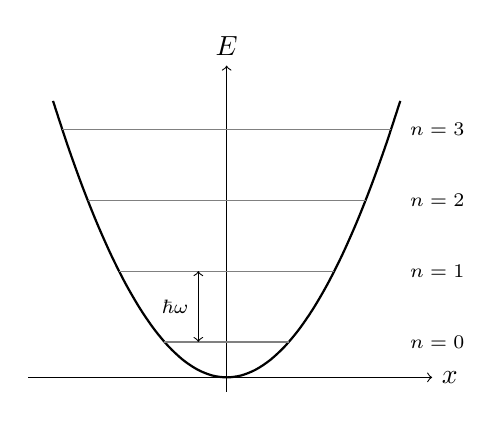
\begin{tikzpicture}[x=0.9cm,y=0.9cm]
  \draw[->] (-2.8,0) -- (2.9,0) node[right] {$x$};
  \draw[->] (0,-0.2) -- (0,4.4) node[above] {$E$};
  \draw[thick,domain=-2.45:2.45,smooth] plot (\x,{0.65*\x*\x});
  \foreach \n in {0,1,2,3} {
    \pgfmathsetmacro{\E}{0.5+\n}
    \pgfmathsetmacro{\w}{sqrt(\E/0.65)}
    \draw[gray] (-\w,\E) -- (\w,\E);
    \node[right,font=\scriptsize] at (2.45,\E) {$n=\n$};
  }
  \draw[<->] (-0.4,0.5) -- (-0.4,1.5) node[midway,left,font=\scriptsize] {$\hbar\omega$};
\end{tikzpicture}
\caption{The potential $\frac12 m\omega^2x^2$ and its lowest four
levels, evenly spaced by $\hbar\omega$ and starting at
$\hbar\omega/2$ above the bottom.}
\label{fig:levels}
\end{figure}

\section{The ground state}

Equation \eqref{eq:ground} is a first-order differential equation in
position space. With $p = -i\hbar\,\mathrm{d}/\mathrm{d}x$,
\begin{equation}
  \left(x + \frac{\hbar}{m\omega}\frac{\mathrm{d}}{\mathrm{d}x}\right)\psi_0(x) = 0 ,
\end{equation}
whose normalised solution is a Gaussian,
\begin{equation}
  \psi_0(x) = \left(\frac{m\omega}{\pi\hbar}\right)^{1/4}
  \exp\!\left(-\frac{m\omega x^2}{2\hbar}\right).
\end{equation}
Its width is the oscillator length $\ell = \sqrt{\hbar/m\omega}$. The
ground state has $\Delta x\,\Delta p = \hbar/2$: it is a state of minimal
uncertainty, the best the uncertainty relation allows. The excited states
follow by applying $\ad$, which in position space gives the Hermite
functions $\psi_n(x) \propto H_n(x/\ell)\,\psi_0(x)$ with the Hermite
polynomials $H_n$.

\section{Coherent states}

The eigenstates $\ket{n}$ do not move: their probability densities are
constant in time, and $\langle x\rangle = 0$ in every one of them. A
classical oscillator, however, swings. The quantum state that swings like
it is an eigenstate of the lowering operator,
\begin{equation}
  a\ket{\alpha} = \alpha\ket{\alpha}, \qquad \alpha\in\mathbb{C},
\end{equation}
which in the number basis reads
\begin{equation}
  \ket{\alpha} = e^{-|\alpha|^2/2}\sum_{n=0}^{\infty}\frac{\alpha^n}{\sqrt{n!}}\,\ket{n}.
\end{equation}
The number of quanta is Poisson distributed with mean $|\alpha|^2$. Under
the time evolution generated by $H$, a coherent state stays coherent,
with $\alpha(t) = \alpha\,e^{-i\omega t}$, so that
\begin{equation}
  \langle x\rangle(t) = \sqrt{2}\,\ell\,|\alpha|\cos(\omega t - \varphi),
\end{equation}
where $\varphi = \arg\alpha$. The Gaussian wave packet keeps its shape
and its minimal uncertainty while its centre follows the classical
trajectory. The light of a laser well above threshold is described by
exactly these states.

\section{Summary}

\begin{itemize}
  \item Writing $H$ with $a$ and $\ad$ turns a differential equation into
        algebra built on $[a,\ad]=1$.
  \item The spectrum $E_n = \hbar\omega(n+\frac12)$ is evenly spaced and
        starts at the zero-point energy $\hbar\omega/2$
        (Fig.~\ref{fig:levels}).
  \item The ground state is a Gaussian of width $\ell$ with minimal
        uncertainty.
  \item Coherent states, the eigenstates of $a$, oscillate like the
        classical particle.
\end{itemize}

\paragraph{Exercises for next week.} (1) Compute $\langle x^2\rangle$ and
$\langle p^2\rangle$ in $\ket{n}$ using only ladder operators, and check
the virial theorem. (2) Show that $\ket{\alpha} = D(\alpha)\ket{0}$ with
$D(\alpha) = \exp(\alpha\ad - \alpha^*a)$. (3) A charged oscillator in a
uniform electric field $\mathcal{E}$: shift $x$ to complete the square and
find the new spectrum.

\end{document}
